\documentclass[12pt, a4paper, openany]{article}
\usepackage[utf8]{inputenc}
\usepackage[T1]{fontenc}
\usepackage{fontspec}
\usepackage{chngcntr}

% LANGUAGE
\usepackage[english]{babel}
% \usepackage{enumitem}  % Enumerate improved
\usepackage[shortlabels]{enumitem}

% MATH / Others
\usepackage{amsmath, amssymb}  % Math symbols
\usepackage{physics}  % \norm and \abs
\usepackage{esvect, cancel}  % Misc., vectors, strikethrough
\usepackage{mhchem}  % Chemistry
\usepackage{siunitx}  % Units SI

% GEOMETRY
\usepackage[
    paper=a4paper,
    top=3cm,
    left=3cm,
    bottom=3cm,
    right=3cm,
    headheight=15pt,
    headsep=12pt,
]{geometry}
\usepackage{parskip}  % Reformat paragraphs, no indent first line
\usepackage{enumitem}  % Enumerate improved
\usepackage{scrextend}  % Indent text with addmargin environment
\usepackage{graphicx}  % Include graphics
\graphicspath{{latex-img}}
\usepackage{caption}  % Caption without figures
\usepackage{float}
\usepackage{multirow}
\usepackage{multicol}


\usepackage{tikz}
\usetikzlibrary{arrows}
\usetikzlibrary{shapes}
\newcommand{\mymk}[1]{%
  \tikz[baseline=(char.base)]\node[anchor=south west, draw,rectangle, rounded corners, inner sep=2pt, minimum size=7mm,
    text height=2mm](char){\ensuremath{#1}} ;}

\newcommand*\circled[1]{\tikz[baseline=(char.base)]{
            \node[shape=circle,draw,inner sep=2pt] (char) {#1};}}

% HYPERLINKS
\usepackage{hyperref}
\hypersetup{
    colorlinks=true,
    linktoc=all,
    linkcolor=blue,
}

\setmonofont[Scale=0.9]{Fira Code}

% HEADERS
\usepackage{fancyhdr}
    \pagestyle{fancy}
    \lhead{Fuzzy Hashing}
    \rhead{L. Grieder / L. Sidjanski}
    \renewcommand{\footrulewidth}{0.4pt}
    \renewcommand{\headrulewidth}{0.4pt}
\usepackage{etoolbox}  % Define chapter page style
    \patchcmd{\chapter}{\thispagestyle{plain}}{\thispagestyle{fancy}}{}{}


% EPFL Logo
\newcommand{\epfllogo}{%
  \begin{figure}[!h]
    \centering
    
\includegraphics[width=0.4\linewidth]{latex-img/logo-epfl.png}
  \end{figure}
}


% TITLE PAGE
\title{Fuzzy Hashing}
\author{Lea Grieder (328216)\\Leila Sidjanski (330810)}
\date{February 2024}

% Capital autoref
\AtBeginDocument{\def\chapterautorefname{Chapitre}}
\AtBeginDocument{\def\sectionautorefname{Section}}
\AtBeginDocument{\def\subsectionautorefname{Sous-Section}}
\AtBeginDocument{\def\figureautorefname{Figure}}

% Custom Commands
\newcommand{\footlink}[2]{\href{#2}{#1}\footnote{#1: \url{#2}}}
\newcommand*{\fullref}[1]{\hyperref[{#1}]{\autoref*{#1} \nameref*{#1}}}

% Counters starts with section number
\counterwithin{figure}{section}
\counterwithin{equation}{section}

\setcounter{tocdepth}{2}

% Colors
\definecolor{myblue}{HTML}{0000ff}
\definecolor{myred}{HTML}{ff0000}
\definecolor{myorange}{HTML}{ff8000}
\definecolor{mygreen}{HTML}{00bf00}

\newcommand{\blue}[1]{{\color{myblue} #1}}
\newcommand{\red}[1]{{\color{myred} #1}}
\newcommand{\orange}[1]{{\color{myorange} #1}}
\newcommand{\green}[1]{{\color{mygreen} #1}}
\newcommand{\black}[1]{{\color{black} #1}}

\newcommand{\definition}[2]{\textbf{#1}: #2}

\begin{document}

% TITLE
\pagestyle{fancy}
\maketitle
\begin{figure}[h]

\includegraphics[scale=0.1]{latex-img/logo-epfl.png}
\centering
\end{figure}
\par\noindent\rule{\textwidth}{0.4pt}
\tableofcontents
\thispagestyle{fancy}
\pagenumbering{arabic}

\newpage

\section{Introduction}

\subsection{Background}
Authentication is the process of confirming the validity of a claimed identity seeking access to a system or resource. Over decades, authentication mechanisms have evolved from basic password systems in the 1960s to advanced methods such as multifactor authentication by the late 2010s, driven by a persistent commitment to combat evolving security risks while enhancing user convenience\cite{ref1}. Various methods such as password-based authentication, certificate-based authentication, one-time passwords, multifactor authentication, and biometric authentication are employed\cite{ref2}.

Biometric authentication, which involves analyzing unique physical characteristics, is often considered more secure than traditional authentication methods due to the difficulty in duplicating biometric traits. This encompasses technologies such as facial recognition, fingerprint recognition, eye recognition, and voice recognition\cite{ref3}.
However, despite the enhanced security of biometric authentication, it is not immune to exploitation. For instance, fingerprints left on surfaces can be copied, or hackers may obtain images of individuals online to deceive authentication systems.
Choosing the right authentication mechanism requires careful consideration of various factors including the necessary security level, ease of use for users, cost implications for setup and ongoing upkeep, as well as the unique risks and vulnerabilities pertinent to the system or data in question. Typically, the requisite level of security steers the selection process; for example, platforms managing sensitive personal information might mandate the use of robust authentication methods, such as biometric verification. The inherent challenge in deploying such secure systems lies in achieving a delicate equilibrium between high security measures and user convenience. The goal is to create an authentication process that is both seamless and efficient, ensuring that access is granted swiftly and accurately to the rightful user without necessitating multiple attempts, thus maintaining a user-friendly experience while upholding the highest security standards.

While advanced biometric systems typically rely on externally visible physical attributes, finger-vein authentication focuses on internal anatomical features, adding a unique layer of security, as they are less prone to replication or theft compared to external characteristics. Nevertheless, it is important to note that finger-vein authentication does not completely eliminate challenges. Despite its emphasis on internal features, attackers can exploit inherent structures in finger veins, such as common patterns among individuals and predictability in acquired data, which poses risks to the authentication process.\\

In light of these considerations, this project is dedicated to authentication using finger-vein features.
This involves utilizing a specialized scanner equipped with two infrared cameras to capture finger veins from different angles.
The registration process involves capturing an image, termed the model image, while the authentication process involves capturing another image, known as the probe image. These images undergo processing through a pipeline designed to extract and align the finger-vein patterns.
The pipeline outputs a feature vector, which is essentially a bitstring, where 0's represent where there are no finger veins, and 1's show where veins are present.
Following this process, the system evaluates whether the feature vector extracted from the probe image sufficiently matches the feature vector of the model image associated with the individual attempting authentication.

\subsection{Extraction Pipeline}\label{sec:extraction-pipeline}

This project extends the work on optimizing a finger-vein recognition pipeline that has demonstrated the lowest \hyperref[def:EER]{Equal Error Rate (EER)} by incorporating a novel hashing step to process the output of the pipeline. The purpose of integrating \hyperref[def:Hash_Function]{Hash Functions} within this context is multifold, but before delving into hash functions, which are central to our project, it's essential to outline the foundation upon which we have built our advancements. This initial context will provide a clearer understanding of the starting point from which our developments began.\\

Simon Sommerhalder and Burcu Yildiz have both made significant contributions to the system. Simon introduced an innovative approach to the alignment of freshly captured images (probe images) with those stored in the system (model images), ensuring the hashing process (following the alignment of the finger) is based on the unique finger-vein pattern rather than how the finger is positioned on the scanner.

Simon has developped a pipeline (see Figure~\ref{pipeline_simon}) to align finger-vein images, enhancing security by eliminating the need to compare the model and probe images side by side. He organized the pipeline into six clear steps:

\begin{enumerate}
    \item \textbf{Masking}: The first step of the pipeline isolates the finger area in the image. This involves creating a mask that outlines the finger, ensuring that subsequent processing focuses solely on the relevant part of the image.

    \item \textbf{Prealignment}: This step involves adjusting the position and orientation of the finger within the image before extracting vein patterns. It's aimed at roughly aligning the image based on the finger's outline, helping to standardize the position of the finger across different scans.

    \item \textbf{Histogram equalization}: To ensure the images have consistent lighting and contrast, this step adjusts the brightness levels. This makes the vein patterns more distinct and comparable across different images.

    \item \textbf{Feature extraction}: Here, the actual vein patterns are identified and extracted from the image. The process converts the visual image into a digital format that represents the presence or absence of veins at specific locations.

    \item \textbf{Postalignment}: After extracting the vein patterns, this step fine-tunes the alignment of the image. It's based on the vein patterns themselves, ensuring that the comparison between model and probe images is as accurate as possible.

    \item \textbf{Distance Calculation}: The final step involves comparing the feature vector of the probe image with that of the model image. This is done using a specific metric to quantify the similarity between the two, ultimately determining if they match closely enough for authentication to succeed.
\end{enumerate} 

\begin{figure}[!h]
    \centering
    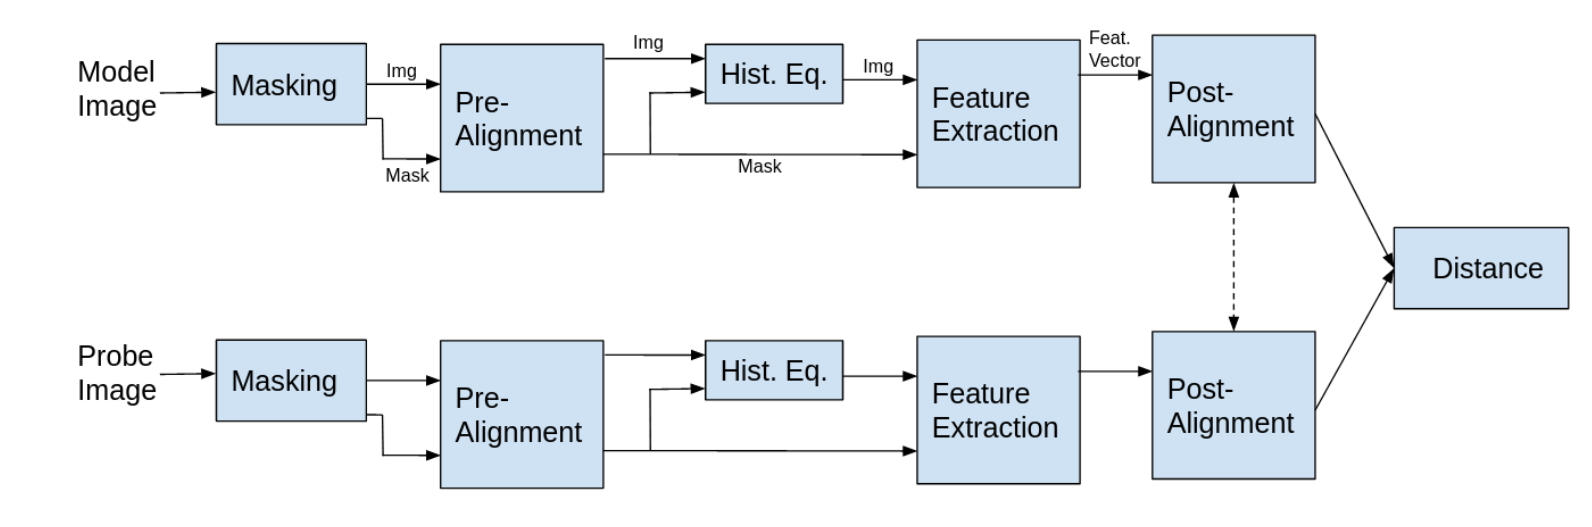
\includegraphics[width=1\linewidth]{latex-img/pipeline_simon.png}
    \caption{Simon's Extraction Pipeline. Compares a single probe image to a model image}
    \label{pipeline_simon}
\end{figure}

Burcu's work on the finger vein authentication project built upon Simon's foundational pipeline, focusing on refining image processing for vein extraction and evaluating different distance calculation methods for authentication. She optimized preprocessing steps, investigated masking and prealignment issues, and tackled reference selection to enhance matching accuracy. A significant part of her contributions involved exploring fuzzy extractors \hyperref[def:Fuzzy_Extractors]{Fuzzy Extractors} to bolster security, conducting a thorough analysis of the dataset to identify and address challenges, and proposing solutions to improve the system's reliability and efficiency.\\

Simon and Burcu explored a variety of function combinations at different stages of the authentication pipeline, aiming to pinpoint the configuration that yields the most favorable outcomes. They utilized the Equal Error Rate (EER) as a benchmark to measure the pipeline's efficacy, focusing on achieving a balance between security and accessibility. This metric, representing the point where the rate of false acceptances (impostor incorrectly granted access) matches the rate of false rejections (legitimate user incorrectly denied), serves as an indicator of the system's reliability and accuracy. The configuration that demonstrated superior performance, leading to the lowest EER and thereby optimizing the process of analyzing and processing images, is showcased in the subsequent figure.

\begin{table}[H]
    \centering
    \caption{EER values for the best pipeline: Edge masking, translation pre-alignment, no pre-processing, no post-
    processing, Miura matching as the post-alignment}
    \begin{tabular}{lc}
    \toprule
    Camera & EER \\
    \midrule
    Camera 1 & 0.041 \\
    Camera 2 & 0.029 \\
    Sum of cameras & 0.030 \\
    \bottomrule
    \end{tabular}
    \label{tab:eervalues_best}
\end{table}

\subsection{Project Overview}

In the progression of our project, building upon the work of Simon and Burcu, we aim to address the inherent variability in biometric data, particularly with finger vein patterns, by considering hash functions. The final objective of the system is to add a hashing step at the end of our established pipeline, prior to the post-alignment phase. The integration of this step serves to enhance security and overall functionality by allowing us to store a hash of each biometric image X in our database, instead of the raw biometric data. Upon receiving a new image Y, we compute hashes for all potential translations of Y, comparing these with the hash of X. Unfortunately, this process is computationally expensive because it requires computing the hash for every possible translation of the image. The purpose of employing a hashing process in this system is multifold:

\begin{itemize}
    \item \textbf{Security}: Hash values can be stored instead of raw biometric data. In the event of a database breach, attackers would find it significantly more challenging to reconstruct the original biometric information from the hashed values due to the one-way nature of hash functions.

    \item \textbf{Consistency}: By focusing on the unique patterns of the biometric trait (like finger-vein patterns) and standardizing how this data is processed and hashed, the system aims to produce consistent hash values for the same individual across different scanning sessions. This is crucial for reliable authentication, ensuring that minor variations in finger placement do not affect the system's ability to recognize the user.

    \item \textbf{Performance}: Hashing biometric data into a compact, fixed-size format facilitates quicker comparison and verification processes. It's more efficient to compare hash values than to perform complex pattern recognition operations on raw biometric images.
\end{itemize}

Traditional hash functions, while pivotal in various data security contexts, generate a unique output for each unique input. This one-to-one mapping means even minor variations in the input — common in biometric data due to natural changes in biological traits or differences in scanning conditions — result in completely different hashes. This sensitivity to input variability poses a challenge in biometric authentication systems, where the goal is to accurately recognize and authenticate an individual despite these natural variations.

Fuzzy hashing stands as a sophisticated solution to this challenge. Unlike traditional hash functions, fuzzy hashing is designed to produce consistent cryptographic keys for inputs that are similar, but not identical. This is particularly advantageous in biometric authentication systems, where it's essential to recognize the same biometric trait across different instances, despite slight variations. The "fuzziness" of this approach allows the system to map these similar inputs to the same or closely related hash values, thereby ensuring that legitimate users are not incorrectly denied access due to minor discrepancies in their biometric data.
Furthermore, the application of fuzzy hashing in our pipeline is instrumental in protecting user privacy. Since the hashed values, rather than raw biometric data, are stored and used for authentication, users' biometric information is safeguarded against potential breaches. Even if hashed values were accessed without authorization, the complexity of fuzzy hashing algorithms makes it extremely challenging to reverse-engineer the original biometric data.\\

The process of our fuzzy hashing algorithm, that we will detail in Section~\ref{sec:Fuzzy Hashing}  begins with a biometric capture, a finger image, which goes through the already developped pipeline~\ref{pipeline_simon} to extract a bitstring. This bitstring undergoes a pre-hashing process, where a subset of significant bits (denoted as vein pixels) is selected based on a permutation keyed by a secure key, resulting in a tuple that significantly reduces the data's dimensionality while preserving its distinguishing features.

Upon generating the fuzzy hash, the next step involves further compressing this hash to prepare it for storage. This compression is achieved through a function, postHash, which maps the tuple to a bitstring of a defined length. The output, essentially a compressed fuzzy hash, exhibits nearly uniform distribution when both the input data and the key are random, enhancing security and storage efficiency.

To further bolster the security of the stored biometric data, this system incorporates \hyperref[def:Fuzzy_Extractors]{Fuzzy Extractors}. The fuzzy extractor framework ensures that even if the stored data is compromised, reconstructing the original biometric data or compromising individual privacy remains computationally infeasible. This is accomplished by generating a secure, random key from the biometric input using a generation process (Gen) and allowing for the reliable reproduction of this key from an approximation of the original input using a reproduction process (Rep), without directly storing the biometric data itself.

In essence, we aim to store the output of the fuzzy extractor, which includes the reproducible cryptographic key and the helper data, instead of the raw biometric data or its direct hash. This method ensures that the stored biometric data is not only compact and efficiently stored but also securely obfuscated, requiring the correct biometric input for any form of decryption or matching to occur.


\section{Theoretical Framework}
Here we explain the theoretical concepts and maths that are explained in our document fuzzytext

\subsection{Biometric Setting}
Explain section 1 of the document (parameterization and representation of biometric data). Explain what biometric data is and its importance in security applications.Explain the transformation of finger pictures into compressed formats for vein pixel extraction (Simon's pipeline). Explain the probability models of section 1: introduce p and the concept of matching biometric captures with an optimal offset, denoted by sigma. to minimize the mismatch probability (p(Xi!=Yi))

\subsection{Concept of Fuzzy Hashing}
Explain what fuzzy hashing is and how it is different from standard hashing in security systems. Describe the PreHash functionality on biometric data, using random permutation to select specific indices corresponding to feature points. Explain the formula for comparing two pre-hashed biometric captures using the hamming weight and the bitwise AND operation to assess the match probability. 
Explain the calculation of the matching score, using the ratio of the hamming weight of the conjunction of two bit strings to their combined hamming weights. Explain what mu is.

\subsection{Compressed Fuzzy Hashing}
Explain how post-hash functions compress the pre-hash bit strings into a more compacted form, maintaining near uniform distribution when inputs are random. Discuss the implications of tis compression on matching probability and introduce the concept of D=2 puissance d to understand the compression ratio and its effects on hash collision probabilities.
Detail the formula calculating the probability of hash matches after compression and the role of mu in determining these probabilities, particularly how it adjusts based on the distribution of biometric captures (same, different, independent)

\subsection{Pre-Hash and Post-Hash Implementation and Analysis}
Explain the algorithm and how we have implemented it

\subsection{Applications in Biometric Macthing}
Illustrate the use of fuzzy hashing in biometric matching by employing the hamming distance to compare hashes, reducing the data required for storing biometric templates and enhancing privacy. Explain how a threhold is defined for determining a match and how false negative rates (FNR) and false positive rates (FPR) are calculated using the cumulative distirbution function (CDF) of the normal distribution, emphasizing the statistical approach to balancing match accuracy and security. 

\subsection{1:N Matching}
Discuss the challenges and strategies for matching a single biometric sample against a large database, focusing on the computational and memory complexities involved. Explain how parameters are adjusted to manage trade offs between time complexity, space complexity, and match probability. Provide insight into the statistical models used for evaluating the performance of 1:N natching systems, including the derviation of FNR and the optimization of parameters for efficient and accurate matching across large datasets. 




\input{parts/Implementation.tex}
\section{Experimental Verifications}

\subsection{Methodology for Assessing Theoretical Values (p, delta, mu)}
% p = probability of a vein pixel being present in a given biometric sample
% delta = probability of differences between two biometric samples 
% mu = theoretical matching probability under optimal conditions (mu depends on p and delta)

\subsection{Analyzing FPR and FNR (Disussion of Results)}
\section{Optimization Strategies}

\subsection{Data Compression Techniques for m=1, d=4}

\subsection{Efficiency Improvement in Hashing Process}
\section{[1:N] Matching and System Evaluation}

\subsection{Implementation of [1:N] Matching}
\subsection{System Performance Evaluation}

\newpage
\newpage
\section{Application: Private and Compact Biometric Matching}
\label{Application: Private and Compact Biometric Matching}

This section delves into the practical application of fuzzy hashing within the realm of biometric matching. Employing the Hamming distance for biometric matching offers a systematic approach by iteratively generating \textit{l} iterations of the \textit{PreHash} function, defined as:

\begin{equation}
    \begin{aligned}
        Hash_{\text{key}}^m &= Hash_{\text{key}_1, \ldots, \text{key}_l}^m(X)\\
        &= (PreHash_{\text{key}_1}^m(X), \ldots, PreHash_{\text{key}_l}^m(X))
    \end{aligned}
\end{equation}

Subsequently, the Hamming distance between the resulting hash values of two biometric samples \(X\) and \(Y\) is calculated as:

\[d_H(Hash_{key}(X), Hash_{key}(Y)) = \# \{i: PreHash_{key_i}(X) \neq PreHash_{key_i}(Y)\}\]

This expression quantifies the instances "i" where the outputs of the \textit{PreHash} function differ between samples \(X\) and \(Y\).

One notable advantage of this approach is the reduction in size of the stored biometric template. Rather than storing \textit{n} pixels, \textit{ml} integers are stored. Additionally, the key renders the reference \textit{PreHash} less privacy-sensitive compared to a biometric template. Specifically, if the key is known, each integer in the hash discloses about \(\frac{1}{p}\) pixels, revealing \(\frac{ml}{p}\) pixels at worst. This disclosure occurs because, with the keys, the hash values can potentially be reverse-engineered to reveal characteristics of the original biometric pattern. The term \(p\)​ reflects the information entropy associated with each bit being a vein (\('1'\)) and thus quantifies the average information content each disclosed pixel conveys when the hash is decoded.

Similarly, when employing the Hamming distance for biometric matching through the iterative generation of \textit{l} iterations of the \textit{PostHash} function, analogous advantages arise. Here, the stored biometric template is condensed to \textit{mld} integers instead of \textit{n} pixels. Furthermore, the key diminishes the sensitivity of the reference \textit{PostHash} in terms of privacy, exposing \(\frac{mld}{p}\) pixels at most if known. Additionally, \textit{PostHash} contributes to leakage reduction.

It's crucial to note that for both scenarios, additional privacy safeguards can be implemented, for instance a restricted access to the key. Hence, the intricacies of the biometric infrastructure must be addressed on a case-by-case basis.

\subsection{Theoretical Foundations of FPR and FNR within Fuzzy Hashing Systems}

Transforming biometric data into a hash, using methods like \textit{PreHash} or its more compact version, \textit{PostHash}, plays a key role in enhancing the system's efficiency and security. This process helps protect privacy, which in turn influences important aspects of the system's performance, such as the \hyperref[def:FNR]{False Negative Rate (FNR)} and the \hyperref[def:FPR]{False Positive Rate (FPR)}. By converting detailed biometric data into a simpler, hashed format, the system not only uses storage space more efficiently but also reduces the chances of unauthorized access to sensitive information. This transformation is crucial for maintaining the integrity of the data and provides a strong line of defense against potential security threats. Additionally, choosing the right techniques for generating these hashes can greatly improve the system's ability to distinguish between authorized and unauthorized users. This means fewer mistakes in the form of false rejections or acceptances, leading to a more accurate and dependable biometric verification process.

We establish a threshold \(t\) to evaluate the match between two biometric samples, \(X\) and \(Y\), by analyzing the Hamming distance between their hash values.
We define that a match is confirmed if the difference between \(l\) (the total iterations) and the Hamming distance is equal to or exceeds the threshold \(t\), expressed as: \[l - d_H(Hash_{\text{key}}(X), Hash_{\text{key}}(Y)) \geq t\]
In contrast, we define there being no match if the following equation holds: \[l - d_H(Hash_{\text{key}}(X), Hash_{\text{key}}(Y)) < t\]

To further refine our understanding, we use statistical methods to approximate this comparison to a normal distribution, allowing us to more accurately calculate the False Negative Rate (FNR). This measure helps us assess how often the system incorrectly fails to recognize a match between the biometric samples when there actually is one. We define:

\begin{equation}
    \label{eq:fnr}
    FNR = \Phi\left( \frac{t - l\mu_{\text{same}}^m}{\sqrt{l\mu_{\text{same}}^m}} \right)
\end{equation}

Here, \(\Phi\) denotes the Cumulative Distribution Function (CDF) of the standard normal distribution, denoted as \(\mathcal{N}(0, 1)\).

In contrast, the False Positive Rate (FPR), the proportion of non-matching biometric samples incorrectly identified as matches by the system, is defined as:

\begin{equation}
    \label{eq:fpr}
    FPR = \Phi\left(- \frac{t - l\mu_{\text{diff}}^m}{\sqrt{l\mu_{\text{diff}}^m}} \right)
\end{equation}

These formulations allow for the evaluation of false match rates based on the standard deviation and mean of the distributions for same and different samples, respectively. The upper bound \(\mu_{same}\) and \(\mu_{diff}\) are defined in Equation \ref{eq:mu}.

For instance, employing \(\Phi(-2.33) \approx 1\%\) as a benchmark, we calculate the threshold (\(t\)) from parameters \(m\) and \(l\) to achieve an FNR of 1\% and an FPR \(\leq 2^{-36} \). The resulting set of parameters is as follows: 

\begin{table}[htbp] 
    \centering
    \begin{tabular}{|c|c|c|c|c|c|c|}
        \hline
        \textit{m} & \textit{l} & \textit{t} & \textit{l}\(\mu_{\text{same}}^m\) & \textit{l}\(\mu_{\text{diff}}^m\) & \textit{FNR} & \textit{FPR} \\
        \hline
        1 & 637 & 118 & 146.6 & 49.2 & 1\% & \(2^{-37}\) \\
        2 & 961 & 34 & 50.0 & 5.7 & 1\% & \(2^{-38}\) \\
        3 & 2569 & 18 & 31.3 & 1.2 & 1\% & \(2^{-41}\) \\
        4 & 8481 & 12 & 23.8 & 0.3 & 1\% & \(2^{-43}\) \\
        5 & 32 999 & 11 & 21.3 & 0.1 & 1\% & \(2^{-51}\) \\
        6 & 140 090 & 10 & 20.8 & 0.0 & 1\% & \(2^{-67}\) \\
        7 & 568 315 & 9 & 19.5 & 0.0 & 1\% & \(2^{-51}\) \\
        8 & 2 841 573 & 11 & 22.4 & 0.0 & 1\% & \(2^{-120}\) \\
        \hline
    \end{tabular}
    \caption{Parameterization Results for FNR and FPR Calculation}
    \label{tab:parameterization}
\end{table}



\subsection{Experimental Derivation of the FPR and FNR for \(m = 1\) and \(d = 4\)}
In this subsection, we will experimentally evaluate the False Positive Rate (FPR) using compression techniques implemented through \textit{PostHash}, specifically compressing to \(D = 16\) (\(d=4\)). The introduction of compression slightly modifies the equations for false positive and false negative rates (Equations \ref{eq:fnr} and \ref{eq:fpr}), necessitating the use of \(q\) in place of \(\mu^m\). Our methodology involves processing our image dataset through a pipeline that initially applies \textit{PreHash} to generate a single index hash (\(m=1\)) for each of the \(l=637\) iterations. Subsequently, \textit{PostHash} compresses these indexes into 4-bit integers. We then compute the normalized Hamming distance between each image pair, with each image represented by \(l \times d\) bits. Lastly, we determine matches based on a specific threshold (\(t\)) tailored to the combined parameters of \(m=1\) and \(l=637\). To facilitate this experiment, we will derive the threshold \(t\) accordingly.
\section{Conclusion}
In this report, we have explored the application of fuzzy hashing to finger-vein biometric authentication, aiming to enhance both security and efficiency. Our investigation included the development and assessment of both the preHash and postHash algorithms, which transform biometric data into secure hash values that maintain consistency despite slight variations in the input data. Got it. The results of the experiments conducted throughout our project generally aligned well with the predicted values. However, as detailed in Section~\ref{sec:Application: Private and Compact Biometric Matching}, some discrepancies arose because certain assumptions of independence may not have been accurate. To address this, we modified our preHash algorithm to ensure that no vein pixel was repeated across the \(l\) iterations of preHash, and performed the first experiment from Table~\ref{tab:theoretical_parameterization_PreHash} using this new algorithm implementation. Despite these efforts, the results did not improve. This could be due to potential errors in the algorithmic implementation, or it may indicate that the chosen approach was not optimal.


\subsection{Challenges and Future Directions}
Throughout our work on this project, we encountered numerous challenges. The first significant difficulty was integrating and building upon the work of previous students. Understanding previously written code can be extremely challenging, highlighting the crucial importance of thorough documentation. We wrote a substantial amount of code for our project, ranging from algorithms such as preHash and postHash to various experimental procedures. Given the initial struggle to comprehend the existing codebase, we prioritized documenting our contributions meticulously. This included adding detailed comments and enhancing the README file to ensure clarity and ease of understanding for future developers. We believe that the comprehensive documentation we have provided will significantly benefit anyone who continues to work on this project, ensuring that our code is accessible and easy to understand.

Another significant challenge was running the experiments. With a dataset of 800 images, each experiment generated four populations of results:

- Population I: Comparisons between same biometric subjects taken from camera 1 (\(1'591\) comparisons).\\
- Population III: Comparisons between same biometric subjects taken from camera 2 (\(1'591\) comparisons).\\
- Population II: Comparisons between different biometric subjects taken from camera 1 (\(37'809\) comparisons).\\
- Population IV: Comparisons between different biometric subjects taken from camera 2 (\(37'809\) comparisons).

This amounted to a total of 78,800 comparisons per experiment, making the runtime extremely long and we spent alot of time waiting for results. We should have addressed this issue earlier but only realized the severity of the runtime problem when conducting experiments for Section~\ref{Application: Private and Compact Biometric Matching}. The extended runtime for multiple iterations of preHash and postHash combinations for each image highlighted the inefficiency. To tackle this, we revisited the previously developed pipeline code and implemented parallel processing. Additionally, we gained access to more powerful ressources (SCITAS\cite{ref4}) to run our code more efficiently. These changes drastically reduced the runtime: experiments that previously took over 24 hours to complete were reduced to just 1 hour.

However, it's important to note that despite the improved runtime, the experiments still consume a lot of resources. Some experiments, such as the last few rows of Table~\ref{tab:theoretical_parameterization_PreHash}, still take between 1 and 4 days to run. This issue can only be further addressed by refining the actual pipeline, specifically the extraction of feature vectors, and by converting the code, which is currently written in Python, to a lower-level language. This transition would likely result in more efficient code execution and reduced resource consumption. The current system requires this especially because future work will be working on a concept called "1:N matching", which adds another layer of complexity to the system, as this process involves comparing a single biometirc input against a database of multiple potential matches to identify the closest match or matches accurately.
\section{Definitions}
\begin{description}
    \item[Equal Error Rate (EER)] \label{def:EER} Metric used to evaluate the performance of a system. It represents the point at which the system's \hyperref[def:FAR]{false acceptance rate (FAR)} equals its \hyperref[def:FRR]{false rejection rate (FRR)}. A lower EER indicates a more accurate and reliable system as it signifies a balanced trade-off between security (minimizing FAR) and usability (minimizing FRR)

    \item[False Acceptance Rate (FAR)] \label{def:FAR} This is the probability of incorrectly accepting an unauthorized user

    \item[False rejection Rate (FRR)] \label{def:FRR} This is the the probability of incorrectly rejecting an authorized user

    \item[Hash Function] \label{def:Hash_Function} A hash function is an algorithm that converts input data of any size to a smaller fixed-size string of characters, which typically acts as a data fingerprint. The output, known as a hash, is unique for different inputs in ideal cases, making hash functions crucial for cryptography, data integrity, and indexing in databases.

    \item[Fuzzy Extractors] \label{def:Fuzzy_Extractors} Fuzzy extractors are cryptographic tools designed to reliably and securely generate a consistent, reproducible cryptographic key from biometric data or other noisy inputs that are inherently inconsistent. They enable the extraction of a stable key from an input that may vary slightly over different measurements, ensuring that even with minor variations, the same key can be reliably regenerated. This process typically involves two main components: a generator that produces a stable key and some public data from an initial input, and a reproducer that can regenerate the original key from a similar but not identical input using the public data.
\end{description}


\newpage

\appendix

\end{document}

